\documentclass[11pt,a4paper]{article}
\usepackage[utf8]{inputenc}
\usepackage[english]{babel}
\usepackage[T1]{fontenc}


\usepackage{amsmath}
\usepackage{amssymb}

\usepackage{float}
\usepackage{graphicx}
\usepackage{picture}
\usepackage{booktabs}
\usepackage{textcomp}
\usepackage{pdflscape}
\usepackage[left=2cm,right=2cm,top=2.5cm,bottom=2cm]{geometry}
\usepackage{listings}
\usepackage{color}
\usepackage[table,xcdraw]{xcolor}
\usepackage[normalem]{ulem}
\useunder{\uline}{\ul}{}

\definecolor{dkgreen}{rgb}{0,0.6,0}
\definecolor{gray}{rgb}{0.5,0.5,0.5}
\definecolor{mauve}{rgb}{0.58,0,0.82}
\newcommand{\comment}[1]{}

\usepackage{fancyhdr}

\pagestyle{fancy}
\fancyhf{}
\rhead{Faculdade de engenharia}
\lhead{Universidade do Porto}
\pagenumbering{arabic}
\pagestyle{fancy}

\lstset{frame=tb,
  aboveskip=3mm,
  escapeinside={<@}{@>},
  belowskip=3mm,
  showstringspaces=false,
  columns=flexible,
  basicstyle={\small\ttfamily},
  numbers=none,
  numberstyle=\tiny\color{gray},
  keywordstyle=\color{blue},
  commentstyle=\color{dkgreen},
  stringstyle=\color{mauve},
  breakatwhitespace=true,
  tabsize=1,    
  extendedchars=true,
  literate={á}{{\'a}}1 {í}{{\'i}}1 {ý}{{\'y}}1 {ř}{{\ˇr}}1  {ã}{{\~a}}1 {é}{{\'e}}1,
}

\title{PGRE - Flow Analysis Problem}
\author{\textit{Alena Tesařová (up201911219)} }
\date{March 2020}

\begin{document}
\begin{center}
\section*{PGRE - Flow Analysis Problem}
\textit{Alena Tesařová (up201911219)}
\end{center}{}
%\maketitle

\begin{enumerate}
    \item \textit{Which is the flow model that characterizes each of these flows in the network?}\\
    Flows identified in the network are:
    \begin{itemize}
        \item \textbf{E-mail }-- client/server,
        \item \textbf{Web access} -- client/server,
         \item \textbf{VoIP} -- the flow for transmitting the digital voice is
essentially peer-to-peer; call setup and teardown is a client/server
flow (a phone needs to talk to a server that understands phone numbers),
         \item \textbf{SAP} - client/server,
          \item \textbf{Backup} - distributed system.
    \end{itemize}{}
    \item\textit{ Which are the important boundaries in the traffic flows of the corporate
network?} \\
The most important boundaries are between: \textit{GW1/ISP1, GW2/ISP1, GW3/ISP1, GW1/ISP2}.
\item \textit{Quantify to approximate values the flows of Email, web access and SAP,
between buildings.}
\begin{itemize}
    \item \textbf{Email flows}
\begin{lstlisting}
GW2/GW3: 
    - around 150 e-mail clients each sending 10 Mbyte and receiving 50 Mbyte
    <@\textcolor{red}{IN}@>: 7500 Mbyte/day
    <@\textcolor{blue}{OUT}@>: 1500 Mbyte/day
Headquarters:
    - around 330 e-mail clients each sending 10 Mbyte and receiving 50 Mbyte
    <@\textcolor{red}{IN}@>: 16500 Mbyte/day
    <@\textcolor{blue}{OUT}@>: 3300 Mbyte/day
\end{lstlisting}
    \item \textbf{Web access}
\begin{lstlisting}
GW2/GW3: 
    - around 150 users each accessing 20 Mbyte of enterprise content 
    - receiving 200 Mbyte external content
    <@\textcolor{red}{IN}@>: 300 Mbyte/day
    <@\textcolor{blue}{OUT}@>: 3000 Mbyte/day
Headquarters:
    - around 330 users each accessing 20 Mbyte of enterprise content 
    - receiving 200 Mbyte external content
    <@\textcolor{red}{IN}@>: 6600 Mbyte/dat
    <@\textcolor{blue}{OUT}@>: 66000 Mbyte/day
\end{lstlisting} 
\item \textbf{SAP}
\begin{lstlisting}
GW2/GW3: 
    - around 10% of 150 users (15 users) makes an average of 20 transactions per day
    - one transaction is 15 kbyte
    Total = 15 * 20 * 15 = 4500 kbyte per day
Headquarters:
    - around 20% of 330 users (66 users) makes an average of 20 transactions per day
    - one transaction is 15 kbyte
    Total = 66 * 20 * 15 = 19800 kbyte per day
\end{lstlisting} 

\end{itemize}{}
\item \textit{Discuss the available bandwidth to access the Internet in the headquarters,
taking into account the values obtained in the previous answer.} \\

In this discussion it is not necessary to take into account SAP transactions because the number is low and it will not influence the result. I understood from the question that we should take into account \textbf{obtained values} from previous question therefore VoIP traffic will not be counted. 

From the assessment we know that Internet connection runs at 100 Mb/s between GW1 and ISP1, 10 Mb/s between GW2 and ISP1 (also GW2 and ISP1) therefore it will firstly be counted the total flow of data going in/out in these flows. 
Firstly, we will sum the total amount of data per day going IN GW2 taking data from previous question: $A_{IN} = 7500 + 300 = 7800$~MB/day, than we will count total amount of data going OUT $A_{OUT} = 1500 + 3000 = 4500$~MB/day. When we summarize everything, we get:
\begin{equation} 
A_{IN} + A_{OUT} = 12300~MB/day\notag
\end{equation}
Now, let's count the theoretical possible usage of Internet in the wire between GW2 and ISP1. It gives 20 MB/s. The working hours are between 9 and 18 (9 hours = 32400 seconds) so the maximum flow is $20 * 32400 = 648000$~MB per day (648~GB). However Ethernet's lines will never be used from 100 \% so we must count on some losses. Considering a loss of 50 \% we get \textbf{324 GB} while we need only 12,3 GB to satisfy Branch A. To conclude, we can see that for line between GW2 and ISP1 there is \textbf{available bandwidth}. For line between GW3 and ISP1 it is the same calculation.
Regrading the line between \textbf{GW1 and ISP1}, we firstly need to calculate the amount of traffic going from GW2 + GW3 that makes 20 \% of total traffic.
\begin{equation} 
A_{IN} + A_{OUT} + B_{IN} + B_{OUT} = 12300 * 2 = 24600~MB/day\notag
\end{equation}
This 24,5 GB makes 20 \% of total traffic on the line. The total utilization is $24.5 * 5 = 122.5$~MB. Ethernet on this line gives as theoretically $100 * 32 400 = 3 240$~GB per day (counting working hours). The real number would be around $3 240 / 2 = 1620$~GB per day. By looking at the result numbers we see that the network was wisely designed and the access to the Internet should be \textbf{available} even for not using the network constantly.
\end{enumerate}{}


\begin{figure}[h]
\centering
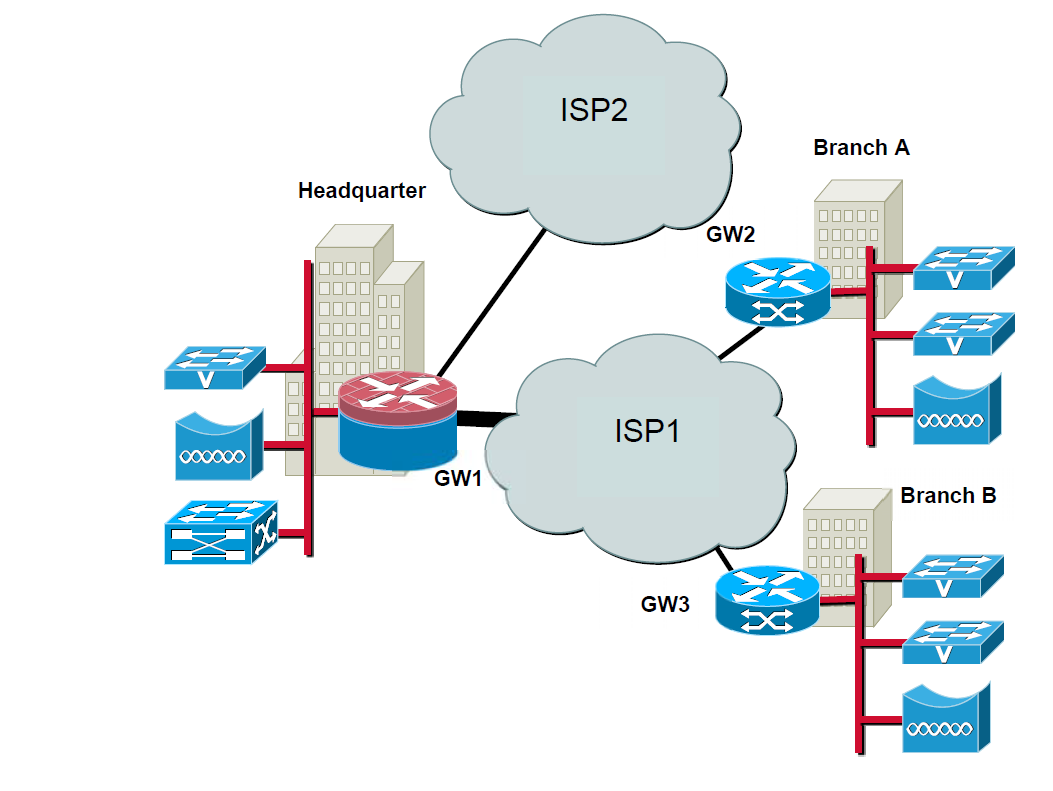
\includegraphics[width=0.6\textwidth]{Capture.PNG}
\caption{Infrastructure of the company}
\label{fig:protokol}
\end{figure}

\end{document}
